\documentclass[a4paper]{article}
\usepackage[14pt]{extsizes} 
\usepackage[T2A]{fontenc}
\usepackage[utf8]{inputenc}
\usepackage{natbib}
\usepackage{graphicx}
\usepackage{amsmath}
\usepackage[english, russian]{babel}
\usepackage{amsmath,amsfonts,amssymb,amsthm,mathtools,mathrsfs}
\usepackage{icomma}
\usepackage{fullpage}
\usepackage{ulem}
\usepackage{eufrak}
\usepackage{setspace}
\usepackage{listings}
\usepackage{indentfirst}
\usepackage[left=2cm,right=1.5cm,top=2cm,bottom=2cm]{geometry}
\usepackage{xcolor}
\usepackage{float}
\usepackage{csquotes}

\setlength{\parindent}{5ex}
\setlength{\parskip}{1em}
\renewcommand{\baselinestretch}{1}

\graphicspath{{images/}}

\definecolor{buzzlightyear}{HTML}{8757A5}
\definecolor{grass}{HTML}{738D06}
\definecolor{literal}{HTML}{F18A2B}
\definecolor{commentcolor}{HTML}{8E908B}

\lstdefinestyle{habrstyle}{
    backgroundcolor=\color{white},   
    commentstyle=\color{commentcolor},
    keywordstyle=\bfseries\color{buzzlightyear},
    numberstyle=\tiny\color{commentcolor},
    stringstyle=\color{grass},
    basicstyle=\ttfamily\footnotesize,
    breakatwhitespace=false,         
    breaklines=true,                 
    captionpos=b,                    
    keepspaces=true,                 
    numbers=left,                    
    numbersep=5pt,                  
    showspaces=false,                
    showstringspaces=false,
    showtabs=false,                  
    tabsize=4
}

\lstset{style=habrstyle}

\begin{document}
    % НАЧАЛО ТИТУЛЬНОГО ЛИСТА
    \begin{center}
        \begin{center}
        \hfill \break
        \normalsize{Санкт-Петербургский государственный политехнический}\\
        \normalsize{университет Петра Великого}\\
        \hfill \break
        \normalsize{\textbf{Высшая школа интеллектуальных систем и}}\\ 
        \normalsize{\textbf{суперкомпьютерных технологий}}\\ 
        \hfill \break
        \hfill \break
        \hfill \break
        \normalsize{Лабораторная работа №4}\\
        \hfill \break
        \hfill \break
        \normalsize{\LARGE Шум}\\
        \end{center}
        \hfill \break
        \hfill \break
        \hfill \break
        \hfill \break
        \hfill \break
        \hfill \break
        \hfill \break
        \hfill \break
        \hfill \break
        \hfill \break
        \begin{flushright}
            \normalsize{Выполнил студент 3-го курса}\\
            \normalsize{группа 3530901/80201}\\
            \normalsize{Матвеец Андрей Вадимович}\\
            \hfill \break
            \normalsize{Преподаватель:}\\
            \normalsize{Богач Наталья Владимировна}\\
        \end{flushright}
        \hfill \break
        \hfill \break
        \hfill \break
        \hfill \break
        \begin{center} Санкт-Петербург\end{center}
        \begin{center}2021\end{center} 
        \thispagestyle{empty}
    \end{center}
    % КОНЕЦ ТИТУЛЬНОГО ЛИСТА
    
    % ОГЛАВЛЕНИЕ
    \newpage
        \tableofcontents
    
    % СПИСОК ИЛЛЮСТРАЦИЙ
    \newpage
         \listoffigures
    
    % СПИСОК ЛИСТИНГОВ     
    \newpage
         \lstlistoflistings   
     
    \newpage
        \section{Часть №1: \texttt{A Soft Murmur}}
            В первой части лабораторной работы нам необходимо скачать файлы с шумом природы, например дождь или морские волны. Выделить из этих сигналов спектры и установить, на какой шум похож каждый сигнал.
            
            В качестве аудиофайлов были выбраны звуки дождя и звуки прибрежных волн. Начнем со звуков дождя.
            
            Прочитаем этот файл и сохраним в переменную \texttt{wave}, после чего выведем полученную аудиодорожку:
            
            \begin{figure}[H]
                \centering
                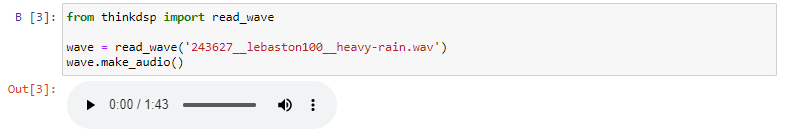
\includegraphics[width=\textwidth]{ex_1_rain_audio.png}
                \caption{Звуки дождя}
                \label{fig:ex_1_rain_audio}
            \end{figure}
            
            После этого выделим сегмент длиной 1с :
            
            \begin{figure}[H]
                \centering
                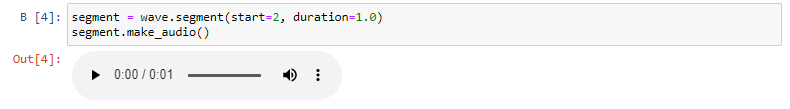
\includegraphics[width=\textwidth]{ex_1_rain_segment_audio.png}
                \caption{Сегмент звуков дождя}
                \label{fig:ex_1_rain_segment_audio}
            \end{figure}
            
            Теперь посмотрим на спектр данного сегмента:
            
\begin{lstlisting}[language=Python, caption= Получение спектра сегмента]
    spectrum = segment.make_spectrum()
    spectrum.plot_power()
    decorate(xlabel='Frequency (Hz)')
\end{lstlisting}               
            
            \begin{figure}[H]
                \centering
                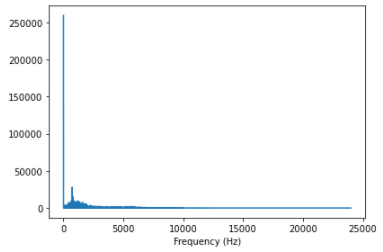
\includegraphics{ex_1_rain_spectr.png}
                \caption{Полученный спектр сегмента}
                \label{fig:ex_1_rain_spectr}
            \end{figure}
            
            Судя по тому, что большей амплитуде соответствует меньшее значение  частоты, то можно сделать вывод о том, что это "красный" или "розовый" шум.
            
            Теперь снова построим спектр сегмента, только в этот раз в логарифмическом масштабе:
            
\begin{lstlisting}[language=Python, caption= Получение логарифмиеского спектра сегмента]
    spectrum.plot_power()
    loglog = dict(xscale='log', yscale='log')
    decorate(xlabel='Frequency (Hz)', **loglog)
\end{lstlisting}               
            
            \begin{figure}[H]
                \centering
                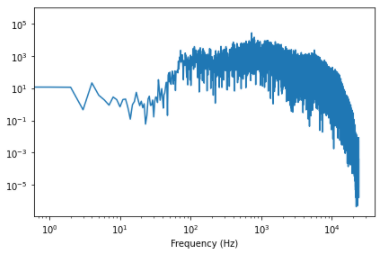
\includegraphics{ex_1_rain_log_spectr.png}
                \caption{Полученный логарифмиеский спектр сегмента}
                \label{fig:ex_1_rain_log_spectr}
            \end{figure}
            
            Далее возьмем какой-нибудь другой сегмент нашего сигнала и произведем все те же самые манипуляции:
            
             \begin{figure}[H]
                \centering
                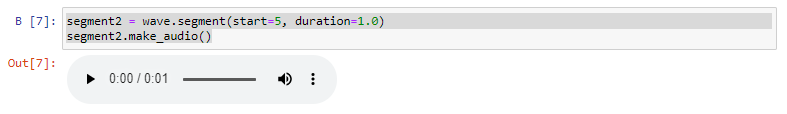
\includegraphics[width=\textwidth]{ex_1_rain_second_segment_audio.png}
                \caption{Другой сегмент звуков дождя}
                \label{fig:ex_1_rain_second_segment_audio}
            \end{figure}
            
            Также сначала получим спектр для нового сегмента:
            
\begin{lstlisting}[language=Python, caption= Получение спектра нового сегмента]
    spectrum2 = segment2.make_spectrum()
    spectrum.plot_power(alpha=0.5)
    spectrum2.plot_power(alpha=0.5)
    decorate(xlabel='Frequency (Hz)',
             ylabel='Amplitude')
\end{lstlisting}               
            
            \begin{figure}[H]
                \centering
                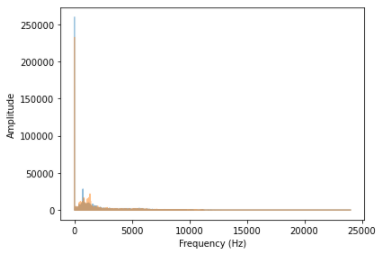
\includegraphics{ex_1_rain_second_spectr.png}
                \caption{Полученный спектр нового сегмента}
                \label{fig:ex_1_rain_spectr}
            \end{figure}
            
            Здесь, на основании полученного спектра можно так же предположить, что это "красный" или "розовый" шум.
            
            Далее так же построим для нового сегмента спектр в логарифмическом масштабе:
            
\begin{lstlisting}[language=Python, caption= Получение логарифмиеского спектра нового сегмента]
    spectrum.plot_power(alpha=0.5)
    spectrum2.plot_power(alpha=0.5)
    decorate(xlabel='Frequency (Hz)',
             ylabel='Amplitude',
             **loglog)
\end{lstlisting}               
            
            \begin{figure}[H]
                \centering
                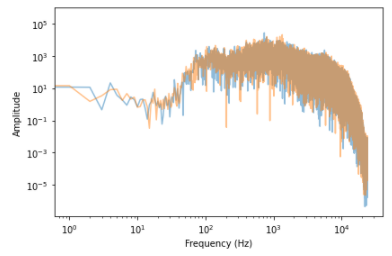
\includegraphics{ex_1_rain_second_log_spectr.png}
                \caption{Полученный логарифмический спектр нового сегмента}
                \label{fig:ex_1_rain_second_log_spectr}
            \end{figure}
            
            По полученным спектрам можно понять, что сигнал сильно не меняется на своем протяжении.
            
            Теперь получим спектограмму для нашего сегмента:
            
\begin{lstlisting}[language=Python, caption= Получение спектограммы для сегмента]
    segment.make_spectrogram(512).plot(high=5000)
    decorate(xlabel='Time(s)', ylabel='Frequency (Hz)')
\end{lstlisting}               
            
            \begin{figure}[H]
                \centering
                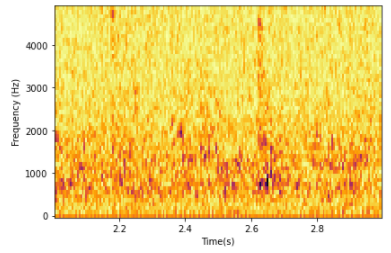
\includegraphics{ex_1_rain_spectogramma.png}
                \caption{Полученная спектограмма сегмента со звуками дождя}
                \label{fig:ex_1_rain_spectogramma}
            \end{figure}
            
            Теперь возьмем второй аудиофайл со звуками волны. Для начала так же сохраним его в переменную \texttt{wave}, после чего выведем полученную аудиодорожку:
            
\begin{figure}[H]
                \centering
                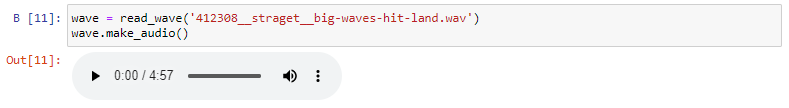
\includegraphics[width=\textwidth]{ex_1_wave_audio.png}
                \caption{Звуки волны}
                \label{fig:ex_1_wave_audio}
            \end{figure}
            
            После этого выделим сегмент длиной 1с :
            
            \begin{figure}[H]
                \centering
                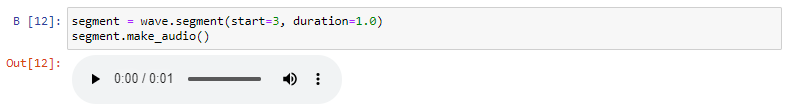
\includegraphics[width=\textwidth]{ex_1_wave_segment_audio.png}
                \caption{Сегмент звуков волны}
                \label{fig:ex_1_wave_segment_audio}
            \end{figure}
            
            Теперь посмотрим на спектр данного сегмента:
            
\begin{lstlisting}[language=Python, caption= Получение спектра сегмента]
    spectrum = segment.make_spectrum()
    spectrum.plot_power()
    decorate(xlabel='Frequency (Hz)')
\end{lstlisting}               
            
            \begin{figure}[H]
                \centering
                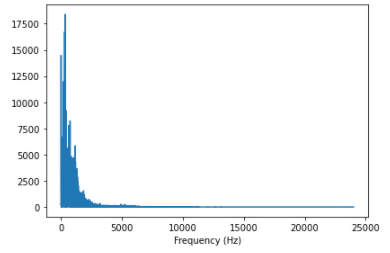
\includegraphics{ex_1_wave_spectr.png}
                \caption{Полученный спектр сегмента}
                \label{fig:ex_1_wave_spectr}
            \end{figure}
            
            Для данного сегмента со звуками волн, судя по тому, что большей амплитуде соответствует меньшее значение частоты, также можно сделать вывод о том, что это "красный" или "розовый" шум.
            
            Теперь снова построим спектр сегмента, только в этот раз в логарифмическом масштабе:
            
\begin{lstlisting}[language=Python, caption= Получение логарифмического спектра сегмента]
    spectrum.plot_power()
    loglog = dict(xscale='log', yscale='log')
    decorate(xlabel='Frequency (Hz)', **loglog)
\end{lstlisting}               
            
            \begin{figure}[H]
                \centering
                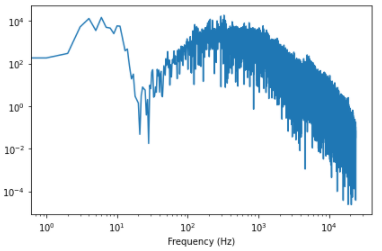
\includegraphics{ex_1_wave_log_spectr.png}
                \caption{Полученный логарифмический спектр сегмента}
                \label{fig:ex_1_wave_log_spectr}
            \end{figure}
            
            Теперь также как и до этого возьмем какой-нибудь другой сегмент нашего сигнала и произведем все те же самые манипуляции:
            
             \begin{figure}[H]
                \centering
                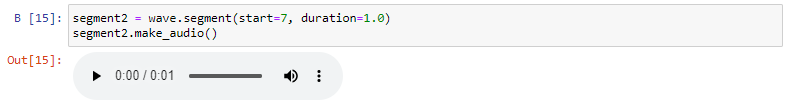
\includegraphics[width=\textwidth]{ex_1_wave_second_segment.png}
                \caption{Другой сегмент звуков дождя}
                \label{fig:ex_1_wave_second_segment}
            \end{figure}
            
            Также сначала получим спектр для нового сегмента:
            
\begin{lstlisting}[language=Python, caption= Получение спектра нового сегмента]
    spectrum2 = segment2.make_spectrum()
    spectrum.plot_power(alpha=0.5)
    spectrum2.plot_power(alpha=0.5)
    decorate(xlabel='Frequency (Hz)',
             ylabel='Amplitude')
\end{lstlisting}               
            
            \begin{figure}[H]
                \centering
                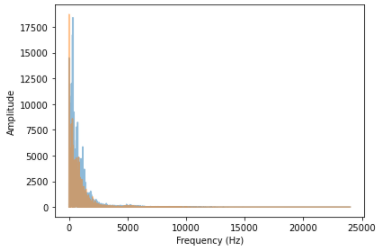
\includegraphics{ex_1_wave_second_spectr.png}
                \caption{Полученный спектр нового сегмента}
                \label{fig:ex_1_rain_spectr}
            \end{figure}
            
            В данном случае как и до этого, на основании полученного спектра можно так же предположить, что это "крансый" или "розовый" шум.
            
            Далее так же построим для нового сегмента спектр в логарифмическом масштабе:
            
\begin{lstlisting}[language=Python, caption= Получение логарифмического спектра нового сегмента]
    spectrum.plot_power(alpha=0.5)
    spectrum2.plot_power(alpha=0.5)
    decorate(xlabel='Frequency (Hz)',
             ylabel='Amplitude',
             **loglog)
\end{lstlisting}               
            
            \begin{figure}[H]
                \centering
                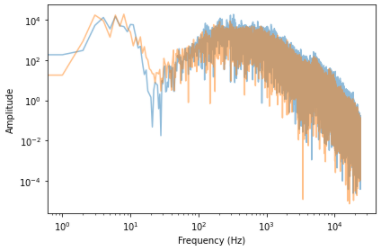
\includegraphics{ex_1_wave_second_log_spectr.png}
                \caption{Полученный логарифмический спектр нового сегмента}
                \label{fig:ex_1_wave_second_log_spectr}
            \end{figure}
            
            По полученным спектрам можно понять, что сигнал со звуками сильно не меняется на своем протяжении, только в первой части есть небольшая разница в амплитудах сигналов.
            
            Теперь получим спектограмму для нашего сегмента:
            
\begin{lstlisting}[language=Python, caption= Получение спектограммы для сегмента]
    segment.make_spectrogram(512).plot(high=5000)
    decorate(xlabel='Time(s)', ylabel='Frequency (Hz)')
\end{lstlisting}               
            
            \begin{figure}[H]
                \centering
                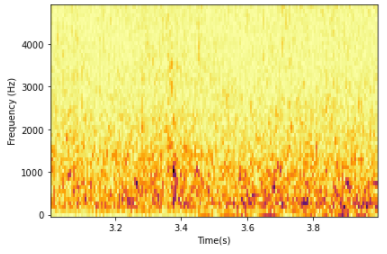
\includegraphics{ex_1_wave_spectogramma.png}
                \caption{Полученная спектограмма сегмента со звуками волны}
                \label{fig:ex_1_wave_spectogramma}
            \end{figure}
    
    \newpage
        \section{Часть №2: Метод Барлетта}
           Во втором пункте лабораторной работы нам необходимо реализовать метод Бартлетта и использовать его для оценки спектра мощности шумового сигнала.
           
           Реализуем метод Бартлетта:
           
\begin{lstlisting}[language=Python, caption= Реализованный метод Бартлетта]
    def bartlett_method(wave, seg_length=512, win_flag=True):
        spectro = wave.make_spectrogram(seg_length, win_flag)
        spectrums = spectro.spec_map.values()
        psds = [spectrum.power for spectrum in spectrums]
        hs = np.sqrt(sum(psds) / len(psds))
        fs = next(iter(spectrums)).fs
        spectrum = Spectrum(hs, fs, wave.framerate)
        return spectrum
\end{lstlisting}      
           
           Проверим данный метод, вызвав его два раза и выведем полученные спектры на одном графике:
           
\begin{lstlisting}[language=Python, caption= Получение спектограммы для сегмента]
    psd = bartlett_method(segment)
    psd2 = bartlett_method(segment2)
    psd.plot_power()
    psd2.plot_power()
    decorate(xlabel='Frequency (Hz)', 
             ylabel='Power', 
             **loglog)
\end{lstlisting}               
            
            \begin{figure}[H]
                \centering
                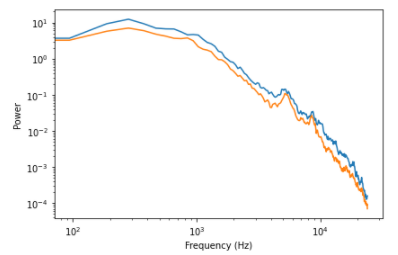
\includegraphics{ex_2_bartlett_spectr.png}
                \caption{Полученные спектры метода Бартлетта}
                \label{fig:ex_2_bartlett_spectr}
            \end{figure}
            
            Проанализировав полученные спектры можно сделать вывод, что в них есть связь между частотой и амплитудой, а сама зависимость нелинейная.

    \newpage
        \section{Часть №3: \texttt{BitCoin}}
            В третьей части лабораторной работы нам необходимо скачать CSV-файл с историческими данными цен на \texttt{BitCoin}. Необходимо вычислить спектр цен \texttt{BitCoin} как функцию времени и установить, на какой шум он больше похож.
            
            Для начала скачаем  CSV-файл с данными цен за \texttt{BitCoin}:
            
\begin{lstlisting}[language=Python, caption= Получение таблицы с данными цен за \texttt{BitCoin}]
    import pandas as pd
    data = pd.read_csv('BTC_USD_2013-10-01_2020-03-26-CoinDesk.csv')
    data
\end{lstlisting}               
            
            \begin{figure}[H]
                \centering
                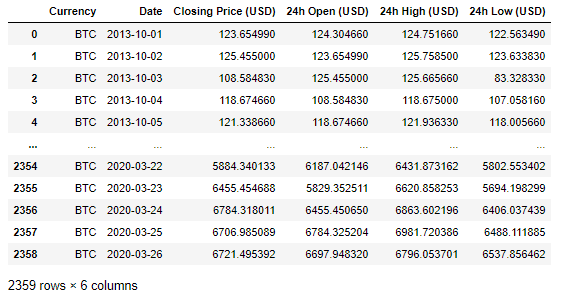
\includegraphics[width=\textwidth]{ex_3_bitcoin_table.png}
                \caption{Таблица с данными цен за \texttt{BitCoin}}
                \label{fig:ex_3_bitcoin_table}
            \end{figure}
            
            Теперь считаем все данные из этой таблицы:
            
\begin{lstlisting}[language=Python, caption= Получение данных из таблицы]
    datac = data['Closing Price (USD)']
    datai = data.index
\end{lstlisting}  
            
            После чего построим \texttt{wave} из полученных данных:
            
\begin{lstlisting}[language=Python, caption= Построение \texttt{wave}]
    from thinkdsp import Wave
    wave = Wave(datac, datai, framerate=1)
    wave.plot()
    decorate(xlabel='Time (days)')
\end{lstlisting}               
            
            \begin{figure}[H]
                \centering
                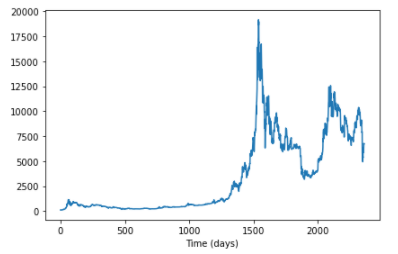
\includegraphics{ex_3_bitcoin_wave.png}
                \caption{\texttt{Wave} на основе данных таблицы}
                \label{fig:ex_3_bitcoin_wave}
            \end{figure}
            
            Наконец, построим логарифмический спектр для наших данных:
            
\begin{lstlisting}[language=Python, caption= Построение логарифмического спектра]
    spectrum = wave.make_spectrum()
    spectrum.plot_power()
    decorate(xlabel='Frequency (1/days)', **loglog)
\end{lstlisting}               
            
            \begin{figure}[H]
                \centering
                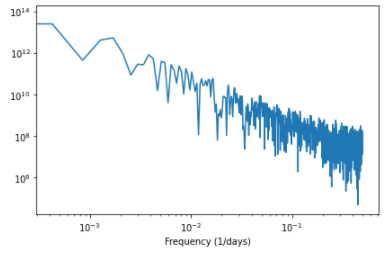
\includegraphics{ex_3_bitcoin_log_spectr.png}
                \caption{Построенный логарифмический спектр}
                \label{fig:ex_3_bitcoin_log_spectr}
            \end{figure}
            
            На основании полученного спектра можно осделать вывод, что это либо «красный», либо «розовый» шум
            
            Посмотрим на наклон полученного спектра:
            
            \begin{figure}[H]
                \centering
                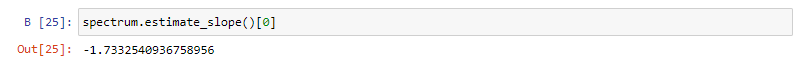
\includegraphics[width=\textwidth]{ex_3_bitcoin_extimate_slope.png}
                \caption{Наклон спектра}
                \label{fig:ex_3_bitcoin_extimate_slope}
            \end{figure}
            
            Наклон получился равным -1,73, в то время как для «красного» шума характерен наклон -2, поэтому можно сделать вывод, что перед нами «розовый» шум.
            
    \newpage
        \section{Часть №4: Счетчик гейгера}
           В четвертом пункте лабораторной работы нам необходимо реализовать класс  \texttt{UncorrelatedPoissonNoise}, наследующий \texttt{Noise} и предоставляющий \texttt{evaluate}. Необходимо сгенерировать случайные величины из распределения Пуассона, а так же пару секунд \texttt{UP} и прослушать. При малых значениях \texttt{amp} звук будет похож на счетчик Гейгера, а при больших на белый шум. Вычислить и напечатать спектр для этих сегналов.
           
           Начнем с написания класса \texttt{UncorrelatedPoissonNoise}:
           
\begin{lstlisting}[language=Python, caption= Построение логарифмического спектра]
    from thinkdsp import Noise
    class UncorrelatedPoissonNoise(Noise):
        def evaluate(self, ts):
            ys = np.random.poisson(self.amp, len(ts))
        return ys
\end{lstlisting} 
           
           После чего сразу создадим сигнал с \texttt{amp} = 0,001 и представим его в виде аудио:
           
           \begin{figure}[H]
                \centering
                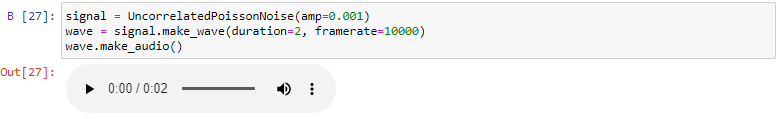
\includegraphics[width=\textwidth]{ex_4_signal_audio.png}
                \caption{Созданный сигнал}
                \label{fig:ex_4_signal_audio}
            \end{figure}
            
            Прослушав полученную аудиодорожку можно сделать вывод, что она очень сильно похожа на звук, издаваемый счетчиком Гейгера.
            
            Сверим ожидаемое количество частиц с полученным:
            
             \begin{figure}[H]
                \centering
                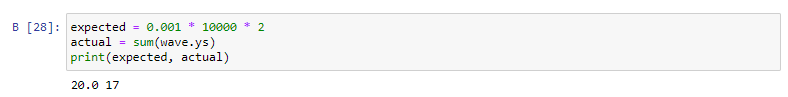
\includegraphics[width=\textwidth]{ex_4_signal_particles .png}
                \caption{Количество частиц}
                \label{fig:ex_4_signal_particles}
            \end{figure}
            
            После этого построим полученные значения:
            
\begin{lstlisting}[language=Python, caption= Визуализация полученных значений]
    wave.plot()
\end{lstlisting}               
            
            \begin{figure}[H]
                \centering
                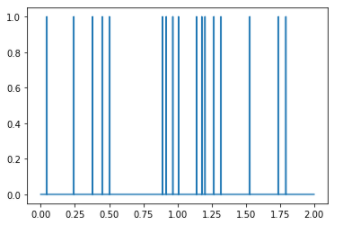
\includegraphics{ex_4_signal_wave_plot.png}
                \caption{Визуализация полученных значений}
                \label{fig:ex_4_signal_wave_plot}
            \end{figure}
            
            Теперь нам необходимо узнать можность спектра:
            
\begin{lstlisting}[language=Python, caption= Мощность спектра]
    spectrum = wave.make_spectrum()
    spectrum.plot_power()
    decorate(xlabel='Frequency (Hz)',
             ylabel='Power',
             **loglog)
\end{lstlisting}               
            
            \begin{figure}[H]
                \centering
                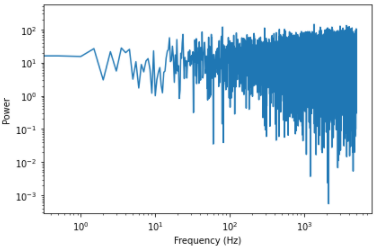
\includegraphics{ex_4_signal_log_spectr.png}
                \caption{Полученная мощность спектра}
                \label{fig:ex_4_signal_log_spectr}
            \end{figure}
            
            Также посмотрим на наклон полученного спектра:
            
            \begin{figure}[H]
                \centering
                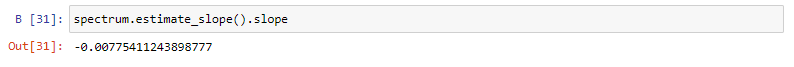
\includegraphics[width=\textwidth]{ex_4_signal_estimate_slope.png}
                \caption{Наклон спектра}
                \label{fig:ex_4_signal_estimate_slope}
            \end{figure}
            
            На основе полученной мощности спекрта и его наклона можно сделать вывод, что наш сигнал представляет собой белый шум
    
    \newpage
        \section{Часть №5: Алгоритм Восса-МакКартни}
            В пятом пункте четвертой лабораторной работы нам необходимо реализовать алгоритм Восса-МакКартни, вычислить спектр и убедиться, что соотношение между мощностью и частотой соответствующие.
            
            Для начала реализуем класс \texttt{voss}:
            
\begin{lstlisting}[language=Python, caption= Класс \texttt{voss}]
    def voss(nrows, ncols=16):
        array = np.empty((nrows, ncols))
        array.fill(np.nan)
        array[0, :] = np.random.random(ncols)
        array[:, 0] = np.random.random(nrows)
        n = nrows
        cols = np.random.geometric(0.5, n)
        cols[cols >= ncols] = 0
        rows = np.random.randint(nrows, size=n)
        array[rows, cols] = np.random.random(n)
        df = pd.DataFrame(array)
        df.fillna(method='ffill', axis=0, inplace=True)
        total = df.sum(axis=1)
        return total.values
\end{lstlisting}       
            
            После чего сразу протестируем его, переведя полученный сигнал в аудио:
            
             \begin{figure}[H]
                \centering
                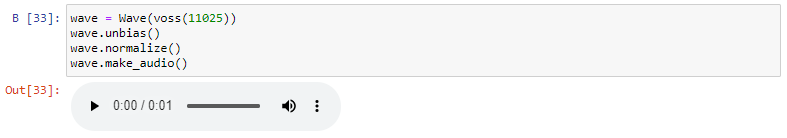
\includegraphics[width=\textwidth]{ex_5_wave_audio.png}
                \caption{Текст класса и перевод в аудио}
                \label{fig:ex_5_wave_audio}
            \end{figure}
            
            Полученная аудиодорожка представляет собой простой шум
            
            Посмотрим как он выглядит:
            
\begin{lstlisting}[language=Python, caption= Просмотр полученной аудиодорожки]
   wave.plot()
\end{lstlisting}               
            
            \begin{figure}[H]
                \centering
                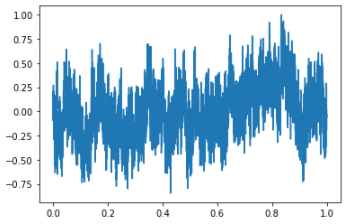
\includegraphics{ex_5_wave_plot.png}
                \caption{Просмотр полученной аудиодорожки}
                \label{fig:ex_5_wave_plot}
            \end{figure}
            
            После этого посмотрим на спектр мощности, чтобы убедиться в правильности зависимости частоты от амплитуды:
            
\begin{lstlisting}[language=Python, caption= Получения спектра мощности]
  spectrum = wave.make_spectrum()
    spectrum.hs[0] = 0
    spectrum.plot_power()
    decorate(xlabel='Frequency (Hz)',
             **loglog)
\end{lstlisting}               
            
            \begin{figure}[H]
                \centering
                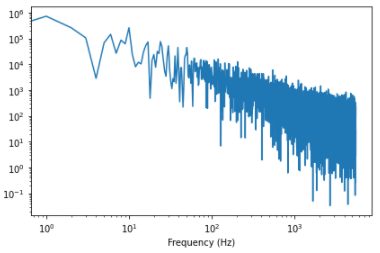
\includegraphics{ex_5_wave_spectr.png}
                \caption{Полученный спектр мощности}
                \label{fig:ex_5_wave_spectr}
            \end{figure}
            
            Также посмотрим на наклон полученного спектра:
            
            \begin{figure}[H]
                \centering
                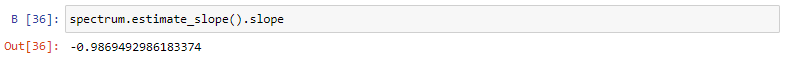
\includegraphics[width=\textwidth]{ex_5_wave_estimate_slope.png}
                \caption{Наклон спектра}
                \label{fig:ex_5_wave_estimate_slope}
            \end{figure}
            
            В результате можно сделать вывод, что полученный нами сигнал является «розовым» шумом, т.к. оценка наклона дает величину близкую к -1.
            
    \newpage
        \section{Выводы}
            В результате выполнения лабораторной работы мы изучили, что такое шум и какие бывают виды шума, а также научились строить спектры мощности шумов. Нами были преобразованы данные по ценам за \texttt{BitCoin} и представлены в виде шума. Кроме того были созданы классы для генерации случайных величин из распределения Пуассона и для реализации алгоритма Восса-МакКартни.
            
\end{document}
